%
% ORIXES DA M�SICA: PATRIMONIO PRIMIXENIO
% ---------------------------------------
\subsection{Patrimonio musical primixenio} \label{sub:patrimonio}

Dentro das fontes organol�xicas que forman parte do patrimonio musical primixenio, atopamos unha serie de instrumentos musicais moi rudimentarios, recuperados en diferentes escavaci�ns arqueol�xicas. A dificultade de co�ecer realmente a organolox�a empregada na prehistoria � debida � utilizaci�n de materiais perecedoiros na construcci�n dos instrumentos musicais, que presentan maior degradaci�n co paso do tempo.

A percusi�n corporal, percutores de pau, pedras de entrechoque, ax�uxeres (pedras, madeiras, l�minas de metal, area, \ldots); raspadores, aer�fonos feitos de canas de �sos; tambores a partires de troncos de �rbores; trompas feitas de cornos de animais e arpas feitas de arcos de frecha, \ldots forman parte do gran cat�logo de instrumentos primixenios da prehistoria.

Pouco podemos dicir en cambio, das fontes musicais. Probablemente empregasen escalas de dous a sete sons, algo semellante �s escalas pentat�nicas. En canto �s melod�as, sabemos que eran curtas e sen complexidades, m�is ben sinxelas, empregando intervalos b�sicos de cuartas, quintas e oitavas. Do estudo etnol�xico comparado de tribus da actualidade, deducimos que � probable que empregasen alg�n tipo de polifon�a simple con bord�n\sidenote{O \textbf{bord�n} consiste nunha nota mantida, soando � vez que a melod�a.} ou heterofon�a\sidenote{A \textbf{heterofon�a}, neste caso fai referencia a d�as li�as mel�dicas con pequenas variantes.}

Alg�ns exemplos organol�xicos deste patrimonio, podemos observalos a continuaci�n.

\begin{multicols}{2}

\begin{Figura}
    \centering
    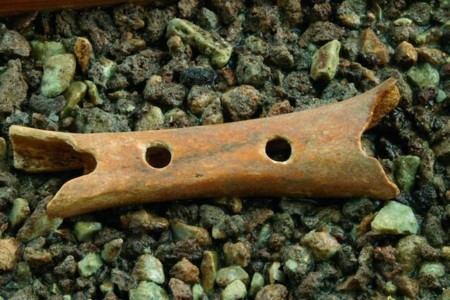
\includegraphics[width=0.9\textwidth]{../figures/ud-00/frauta-oso.jpg}
    \captionof{figure}{Aer�fono prehist�rico.}
    \label{fig:frauta-oso}
\end{Figura}

\end{multicols}
